\documentclass[aspectratio=169,10pt]{beamer}

\usepackage[T1]{fontenc}
\usepackage{lmodern}
\usepackage{booktabs}
\usepackage{tabularx}
\usepackage{tikz}
\usetikzlibrary{arrows.meta,positioning}

\definecolor{Forest}{HTML}{153C32}
\definecolor{Mint}{HTML}{C9F0DC}
\definecolor{Cream}{HTML}{F8F6EF}
\definecolor{Rust}{HTML}{B65738}
\definecolor{Muted}{HTML}{64706C}

\setbeamercolor{normal text}{fg=Forest,bg=Cream}
\setbeamercolor{structure}{fg=Forest}
\setbeamercolor{frametitle}{fg=Forest,bg=Cream}
\setbeamercolor{title}{fg=Forest}
\setbeamercolor{subtitle}{fg=Muted}
\setbeamercolor{block title}{fg=Forest,bg=Mint}
\setbeamercolor{block body}{fg=Forest,bg=Mint!32!Cream}
\setbeamercolor{alerted text}{fg=Rust}
\setbeamertemplate{navigation symbols}{}
\setbeamertemplate{itemize item}{\color{Rust}$\blacktriangleright$}
\setbeamertemplate{itemize subitem}{\color{Forest}$\bullet$}
\setbeamertemplate{footline}{%
  \leavevmode\hbox{%
    \begin{beamercolorbox}[wd=.82\paperwidth,ht=2.6ex,dp=1.1ex,leftskip=1em]{author in head/foot}%
      \color{Muted}\scriptsize Digital Professor: interaction and evidence integration
    \end{beamercolorbox}%
    \begin{beamercolorbox}[wd=.18\paperwidth,ht=2.6ex,dp=1.1ex,rightskip=1em plus1fil]{date in head/foot}%
      \color{Muted}\scriptsize\hfill\insertframenumber/\inserttotalframenumber
    \end{beamercolorbox}}}
\setbeamertemplate{frametitle}{\vspace{.35em}\insertframetitle\par\vspace{.15em}\hrule height .4pt}

\newcommand{\good}[1]{\textcolor{Forest}{\textbf{#1}}}
\newcommand{\risk}[1]{\textcolor{Rust}{\textbf{#1}}}

\title{Digital Professor: Interaction Integration}
\subtitle{What the module provides and how it connects the full system}
\author{Jonathan Ma}
\date{October 2026}

\begin{document}

\begin{frame}[plain]
  \vfill
  {\usebeamerfont{title}\color{Forest}\LARGE\inserttitle\par}
  \vspace{.5em}
  {\color{Muted}\large\insertsubtitle\par}
  \vspace{1.5em}
  {\color{Rust}\rule{2.2cm}{2pt}}\par
  \vspace{1.2em}
  {\small\insertauthor\hfill\insertdate}
  \vfill
\end{frame}

\begin{frame}{What my module provides}
\begin{columns}[T,onlytextwidth]
\column{.49\textwidth}
\begin{block}{Shared records}
\begin{itemize}
\item Course, session, turn, action, and evidence IDs
\item Structured Student Evidence
\item Confirmation and revision history
\item Retrieved-source and delivery records
\end{itemize}
\end{block}
\column{.49\textwidth}
\begin{block}{Integration functions}
\begin{itemize}
\item Route data between specialized components
\item Validate input before downstream use
\item Prepare consistent chat, speech, math, and avatar output
\item Record the full interaction for evaluation
\end{itemize}
\end{block}
\end{columns}
\vspace{.5em}
\centering
\good{Student Evidence:} a structured, traceable record of what the student submitted, how it was interpreted, and what help preceded it.
\end{frame}

\begin{frame}{What my module guarantees}
\begin{columns}[T,onlytextwidth]
\column{.49\textwidth}
\begin{block}{The layer owns}
\begin{itemize}
\item Shared identifiers and data formats
\item Routing between components
\item Student Evidence validation
\item Confirmation, revision, and delivery history
\end{itemize}
\end{block}
\column{.49\textwidth}
\begin{block}{It must always}
\begin{itemize}
\item Preserve original student work
\item Confirm meaning-changing notation
\item Separate student, source, system, and tool content
\item Link revisions without overwriting attempts
\item Keep output consistent across channels
\item Fall back to chat when another service fails
\end{itemize}
\end{block}
\end{columns}
\vspace{.5em}
\centering
Every response must trace back to confirmed student work and supplied course sources.
\end{frame}

\begin{frame}{What my module receives and returns}
\small
\begin{columns}[T,onlytextwidth]
\column{.49\textwidth}
\begin{block}{Inputs}
\begin{itemize}
\item Verified syllabus course profile
\item Retrieved lecture passages and pages
\item Text, voice, handwriting, images, equations, or files
\item Recognition alternatives and student corrections
\item Current problem, prior attempts, and requested help
\item Available delivery channels and system rules
\end{itemize}
\end{block}
\column{.49\textwidth}
\begin{block}{Outputs}
\begin{itemize}
\item Course workspace linked to indexed notes
\item Validated Student Evidence
\item Student Evidence with retrieved sources
\item Confirmation or processing status
\item Chat, speech, math, citation, and avatar package
\item Complete interaction history and measurements
\end{itemize}
\end{block}
\end{columns}
\vspace{.35em}
\centering
Every handoff includes identity, source, status, and validation. Missing information stays missing.
\end{frame}

\begin{frame}{Core output: Student Evidence}
\small
\begin{columns}[T,onlytextwidth]
\column{.49\textwidth}
\begin{block}{What the student provided}
\begin{itemize}
\item Original submission and modality
\item Confirmed transcription
\item Equations, steps, and answer
\item Explanation and uncertainty
\end{itemize}
\end{block}
\begin{block}{Where it belongs}
Student, course, problem, concept, turn, and time.
\end{block}
\column{.49\textwidth}
\begin{block}{How it relates}
\begin{itemize}
\item Prompt or hint that elicited it
\item Attempt and revision links
\item Prior evidence
\item Assistance received
\end{itemize}
\end{block}
\begin{block}{How it was processed}
Recognition confidence, unresolved alternatives, edits, provider, latency, and cost.
\end{block}
\end{columns}
\vspace{.3em}
\centering
The raw submission remains immutable; interpretations and revisions stay separately traceable.
\end{frame}

\begin{frame}{What my module does: setup and input}
\centering
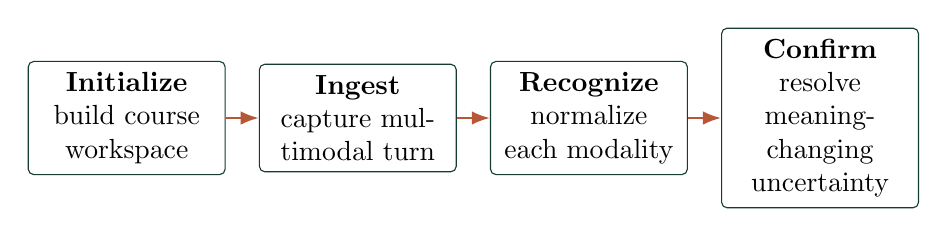
\begin{tikzpicture}[
  node distance=.42cm,
  box/.style={draw=Forest,rounded corners=2pt,fill=white,align=center,
    text width=2.22cm,minimum height=1.15cm,inner sep=4pt},
  arrow/.style={-{Latex[length=2.3mm]},thick,draw=Rust}]
\node[box](receive){\textbf{Initialize}\\build course workspace};
\node[box,right=of receive](route){\textbf{Ingest}\\capture multimodal turn};
\node[box,right=of route](assess){\textbf{Recognize}\\normalize each modality};
\node[box,right=of assess](confirm){\textbf{Confirm}\\resolve meaning-changing uncertainty};
\draw[arrow](receive)--(route);\draw[arrow](route)--(assess);\draw[arrow](assess)--(confirm);
\end{tikzpicture}
\vspace{.8em}
\begin{columns}[T,onlytextwidth]
\column{.49\textwidth}
\begin{block}{\texttt{initialize\_course\_workspace}}
Connect verified syllabus fields to indexed lecture notes.
\end{block}
\begin{block}{\texttt{receive\_submission}}
Store every input modality in one submission record.
\end{block}
\column{.49\textwidth}
\begin{block}{\texttt{route\_recognition}}
Run allowed recognition tools and retain alternatives and confidence.
\end{block}
\begin{block}{\texttt{apply\_confirmation}}
Keep the original reading and the student's correction.
\end{block}
\end{columns}
\end{frame}

\begin{frame}{What my module does: ground and deliver}
\centering
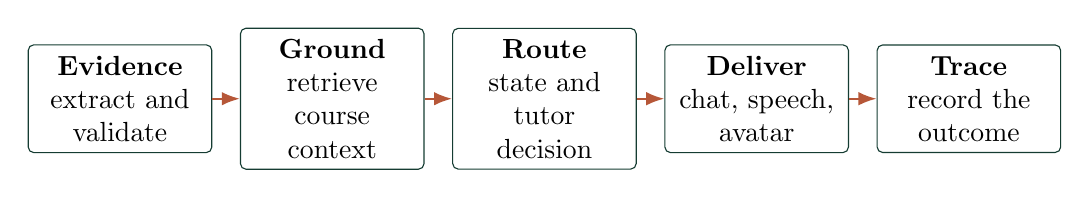
\begin{tikzpicture}[
  node distance=.35cm,
  box/.style={draw=Forest,rounded corners=2pt,fill=white,align=center,
    text width=2.05cm,minimum height=1.15cm,inner sep=4pt},
  arrow/.style={-{Latex[length=2.3mm]},thick,draw=Rust}]
\node[box](extract){\textbf{Evidence}\\extract and validate};
\node[box,right=of extract](link){\textbf{Ground}\\retrieve course context};
\node[box,right=of link](validate){\textbf{Route}\\state and tutor decision};
\node[box,right=of validate](publish){\textbf{Deliver}\\chat, speech, avatar};
\node[box,right=of publish](trace){\textbf{Trace}\\record the outcome};
\draw[arrow](extract)--(link);
\draw[arrow](link)--(validate);
\draw[arrow](validate)--(publish);
\draw[arrow](publish)--(trace);
\end{tikzpicture}
\vspace{.8em}
\begin{itemize}
\item \texttt{publish\_evidence}: validate the student record and notify the next component.
\item \texttt{request\_context}: retrieve relevant lecture passages and pages.
\item \texttt{route\_decision}: send evidence, sources, and the current understanding estimate.
\item \texttt{prepare\_delivery}: create consistent chat, math, speech, citation, and avatar content.
\item \texttt{record\_delivery}: record what the student received and how they responded.
\end{itemize}
\end{frame}

\begin{frame}[shrink=3]{How my module ties everything together}
\centering
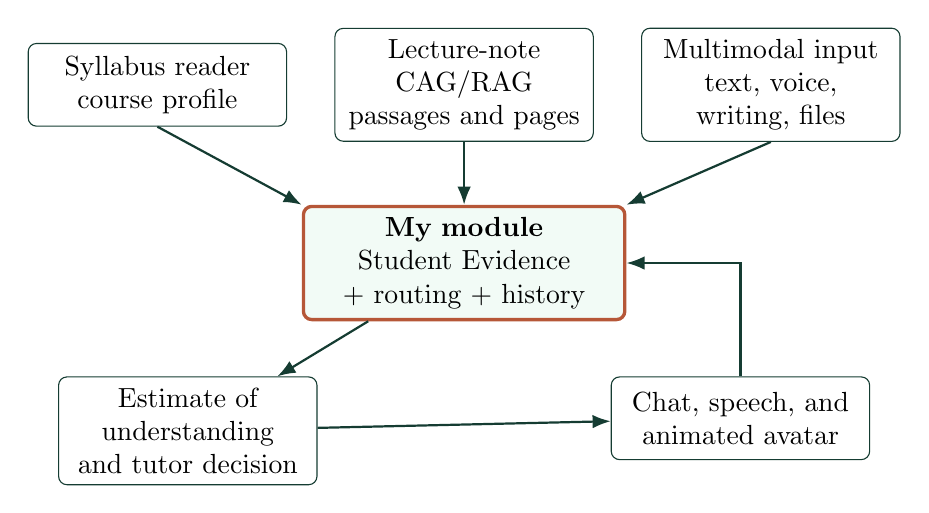
\begin{tikzpicture}[
  node distance=.45cm and .6cm,
  box/.style={draw=Forest,rounded corners=3pt,fill=white,align=center,
    text width=3cm,minimum height=1.05cm,inner sep=4pt},
  core/.style={draw=Rust,very thick,rounded corners=3pt,fill=Mint!25,align=center,
    text width=3.8cm,minimum height=1.2cm,inner sep=4pt},
  arrow/.style={-{Latex[length=2.3mm]},thick,draw=Forest}]
\node[box](syllabus){Syllabus reader\\course profile};
\node[box,right=of syllabus](rag){Lecture-note CAG/RAG\\passages and pages};
\node[box,right=of rag](multi){Multimodal input\\text, voice, writing, files};
\node[core,below=8mm of rag](integration){\textbf{My module}\\Student Evidence + routing + history};
\node[box,below left=7mm and -2mm of integration](decision){Estimate of understanding and tutor decision};
\node[box,below right=7mm and -2mm of integration](delivery){Chat, speech, and animated avatar};
\draw[arrow](syllabus.south)--(integration.north west);
\draw[arrow](rag)--(integration);
\draw[arrow](multi.south)--(integration.north east);
\draw[arrow](integration)--(decision);
\draw[arrow](decision)--(delivery);
\draw[arrow](delivery.north)|-(integration.east);
\end{tikzpicture}
\vspace{.35em}
\small
\begin{itemize}\setlength{\itemsep}{.15em}
\item Course and student data enter through one validated interaction record.
\item One approved action drives chat, speech, mathematics, and avatar delivery.
\item The response returns as the next Student Evidence event.
\end{itemize}
\end{frame}

\begin{frame}{General tutoring workflow mapped to my module}
\small
\begin{tabularx}{\textwidth}{@{}p{.29\textwidth}X@{}}
\toprule
\textbf{Tutoring stage} & \textbf{What my module does} \\
\midrule
1. Establish course context & Build the course workspace from verified syllabus fields and indexed lecture notes. \\
2. Elicit student thinking & Present a question or task, then capture text, voice, handwriting, files, explanation, and uncertainty. \\
3. Interpret the response & Run recognition, confirm meaning-changing notation, and publish a Student Evidence event. \\
4. Select an intervention & Add retrieved course passages and send evidence, prior help, and source pages to the tutoring decision layer. \\
5. Present the intervention & Turn the approved question, hint, retry, or explanation into consistent chat, speech, math, citations, and avatar cues. \\
6. Reassess and continue & Link the student's revision, comprehension check, or transfer answer to the prior action and start the next cycle. \\
\bottomrule
\end{tabularx}
\vspace{.45em}
\centering
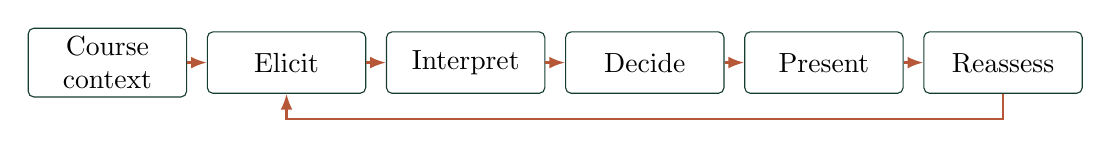
\begin{tikzpicture}[node distance=.25cm,
box/.style={draw=Forest,rounded corners=2pt,fill=white,align=center,text width=1.8cm,minimum height=.78cm,inner sep=3pt},
arrow/.style={-{Latex[length=2mm]},thick,draw=Rust}]
\node[box](context){Course context};
\node[box,right=of context](elicit){Elicit};
\node[box,right=of elicit](interpret){Interpret};
\node[box,right=of interpret](decide){Decide};
\node[box,right=of decide](present){Present};
\node[box,right=of present](reassess){Reassess};
\draw[arrow](context)--(elicit);\draw[arrow](elicit)--(interpret);\draw[arrow](interpret)--(decide);\draw[arrow](decide)--(present);\draw[arrow](present)--(reassess);
\draw[arrow](reassess.south) -- ++(0,-.32) -| (elicit.south);
\end{tikzpicture}
\end{frame}

\begin{frame}[shrink=5]{How it works in one tutoring turn}
\centering
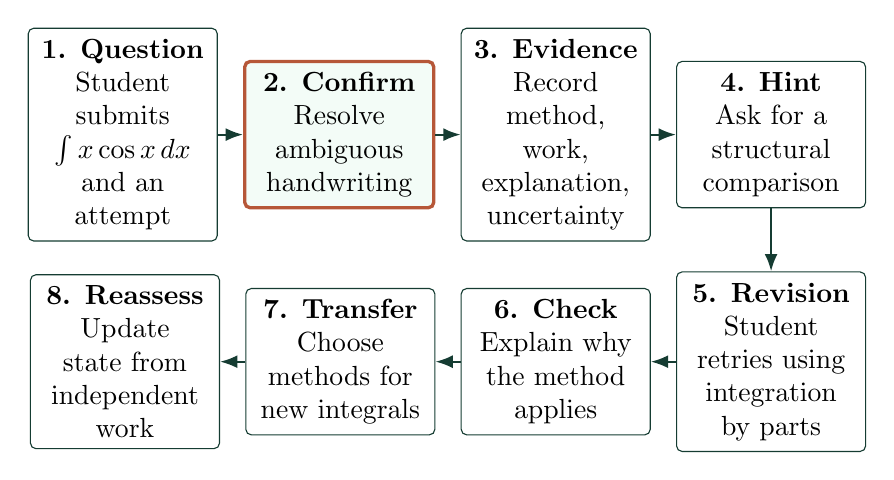
\begin{tikzpicture}[
  node distance=.32cm,
  box/.style={draw=Forest,rounded corners=2pt,fill=white,align=center,
    text width=2.12cm,minimum height=1.2cm,inner sep=4pt},
  guard/.style={draw=Rust,very thick,rounded corners=2pt,fill=Mint!22,align=center,
    text width=2.12cm,minimum height=1.2cm,inner sep=4pt},
  arrow/.style={-{Latex[length=2.2mm]},thick,draw=Forest}]
\node[box](question){\textbf{1. Question}\\Student submits $\int x\cos x\,dx$ and an attempt};
\node[guard,right=of question](confirm){\textbf{2. Confirm}\\Resolve ambiguous handwriting};
\node[box,right=of confirm](evidence){\textbf{3. Evidence}\\Record method, work, explanation, uncertainty};
\node[box,right=of evidence](hint){\textbf{4. Hint}\\Ask for a structural comparison};
\draw[arrow](question)--(confirm);\draw[arrow](confirm)--(evidence);\draw[arrow](evidence)--(hint);
\node[box,below=8mm of hint](revision){\textbf{5. Revision}\\Student retries using integration by parts};
\node[box,left=of revision](check){\textbf{6. Check}\\Explain why the method applies};
\node[box,left=of check](transfer){\textbf{7. Transfer}\\Choose methods for new integrals};
\node[box,left=of transfer](reassess){\textbf{8. Reassess}\\Update state from independent work};
\draw[arrow](hint)--(revision);\draw[arrow](revision)--(check);\draw[arrow](check)--(transfer);\draw[arrow](transfer)--(reassess);
\end{tikzpicture}
\vspace{.65em}
\begin{columns}[T,onlytextwidth]
\column{.49\textwidth}
\begin{block}{System actions presented}
Question, targeted hint, retry request, explanation when needed, comprehension check, and transfer problems.
\end{block}
\column{.49\textwidth}
\begin{block}{Student responses captured}
Initial approach, handwriting, intermediate work, explanation, uncertainty, corrected attempt, and transfer answer.
\end{block}
\end{columns}
\end{frame}

\begin{frame}{How it ties into tutoring decisions}
\small
\begin{columns}[T,onlytextwidth]
\column{.48\textwidth}
\begin{block}{Integration layer sends}
\begin{itemize}
\item Validated Student Evidence event
\item Problem, concept, and requested help
\item Confirmed work and uncertainty
\item Prior attempts and assistance
\item Retrieved passages and page IDs
\end{itemize}
\end{block}
\column{.49\textwidth}
\begin{block}{Decision layer returns}
\begin{itemize}
\item Question, hint, retry, explanation, or check
\item Student-facing text and mathematics
\item Amount of solution to show
\item Sources and expected response
\item Tool request and human-review trigger
\end{itemize}
\end{block}
\end{columns}
\vspace{.15em}
\centering
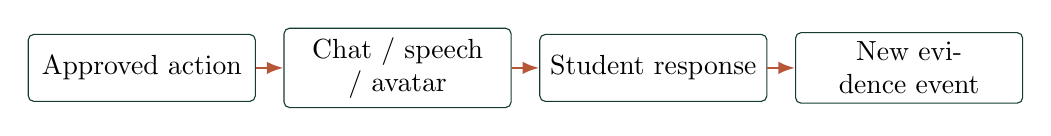
\begin{tikzpicture}[node distance=.35cm,
box/.style={draw=Forest,rounded corners=2pt,fill=white,align=center,text width=2.65cm,minimum height=.85cm},
arrow/.style={-{Latex[length=2.1mm]},thick,draw=Rust}]
\node[box](decision){Approved action};
\node[box,right=of decision](delivery){Chat / speech / avatar};
\node[box,right=of delivery](response){Student response};
\node[box,right=of response](event){New evidence event};
\draw[arrow](decision)--(delivery);\draw[arrow](delivery)--(response);\draw[arrow](response)--(event);
\end{tikzpicture}
\end{frame}

\begin{frame}{What comes next}
\begin{enumerate}
\item Agree on shared identifiers and data formats.
\item Define handoffs for course profiles, retrieved notes, student turns, and delivery.
\item Build one end-to-end sourced tutoring path.
\item Add handwriting confirmation and revision tracking.
\item Compare chat, speech, and avatar delivery for consistency, latency, and recovery.
\end{enumerate}
\vspace{.55em}
\begin{block}{First implementation target}
Course setup $\rightarrow$ sourced tutoring turn $\rightarrow$ validated evidence $\rightarrow$ delivery $\rightarrow$ linked response.
\end{block}
\end{frame}

\begin{frame}{Potential risks and problems}
\small
\begin{tabularx}{\textwidth}{@{}p{.29\textwidth}X@{}}
\toprule
\textbf{Risk} & \textbf{Why it could slow or block progress} \\
\midrule
No shared data contract & Components break if identifiers, statuses, or field meanings drift. \\
Conflicting course context & Syllabus fields and retrieved notes may be missing, stale, or contradictory. \\
Real-time latency & Recognition, retrieval, generation, speech, and animation may be too slow together. \\
Channel inconsistency & Chat, spoken math, and avatar delivery may communicate different meanings. \\
Confirmation burden & Too little corrupts evidence; too much interrupts tutoring. \\
Privacy and dependency & Voice, student work, and external providers create retention and service risks. \\
\bottomrule
\end{tabularx}
\vspace{.4em}
\centering
\risk{Immediate dependency:} agree on shared data formats and handoff rules before each subsystem evolves independently.
\end{frame}

\end{document}
